\chapter{Cross-lingual Word Embedding without Parallel Data}
Proposed cross-lingual embedding learning requires several thousands of word pairs as anchors to learn the mapping with good generalization ability to predict for unseen word. But as for low-source language, dictionary of good quality is not readily available. This motivates more and more works on unsupervised cross-lingual word embedding learning, if the unsupervised method works, the word-level or grammar-level properties will be better captured, since it enables the knowledge transfer for those less-studied languages.

%\begin{figure}[t]
%	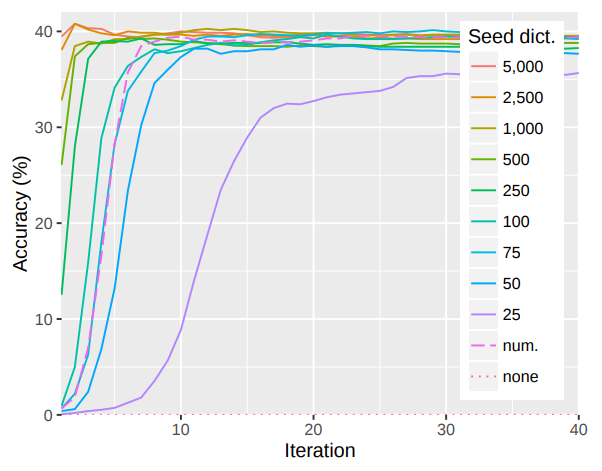
\includegraphics[width=12cm]{iter1}
%	\centering
%	\caption{Accuracy on bilingual lexicon induction}
%\end{figure}	
%
%
%
%
%
%
%
\section{Initialization}
 \cite{vulic2016role} shows that a seed dictionary of at least hundreds are need for the model to generalize. \cite{DBLP:journals/corr/abs-1801-06126}
 proposed an approach which first use PCA to realize an approximate alignment, then use mini-batch cycle iterative closest point to learn the mapping.  
\cite{zhang2017adversarial} proposed an adversarial autoencoder, using the generator $G$ to implement the mapping so that the transformed source embedding similar to the corresponding target embedding, and the discriminator $D$ strives to distinguish the target embedding from the transformed source embedding. \cite{conneau2017word} simplifies the structure and proposed an unsupervised criterion that is highly correlated with the quality of the mapping which can be used as stop criterion and to select the best hyper-parameters.
%
%As it can be clearly observed from the figure below that, the self learning algorithm can effectively learn the mapping between the source and target distribution even starts with a small dictionary size and the final accuracy when the algorithm converges are nearly the same level. However when start randomly without any support of dictionary, the framework does not work. In order to realize a fully unsupervised learning, we need to design heuristics to build the seed dictionary.
%
%For total unsupervised learning, there is no direct alignment between the languages. 	The most challenge for unsupervised learning is the initialization. As proved in the experiment of \cite{}, the self-learning framework can work even with a small dictionary set, however the model cannot work without such dictionary as hint.  So it is important to find heuristic methods to initialize the model.
%
%Several models are proposed:
%Based on matrices ${M_E = EE^T}$, ${M_F = FF^T}$, we can exploit latent information to reduce the mismatch. Assume that, the words in the source and target set are most common. For a specific word, the corresponding line in ${M_E}$ demonstrates the distribution of similarity in the source vocabulary. ${M_E}$, ${M_F}$ can be nearly equivalent up to a permutation of the words. 
%Instead of explore all the probability of permutation, he first sorts the values in each row of ${M_F}$ and ${M_E}$
%
%Assume the SVD of ${E = USV^T}$,  the similarity ${M_E = US^2U^T}$. In practice, he computed sorted ${1}$, ${2}$	yielding the matrix ${E^{\prime}}$ , ${F^{\prime}}$ and used to build the initial solution for self-learning.

\subsection{Iterative Closest Point Method}

The method assumes that many language pairs share some principle axes of variation. For each language, first select most frequent word vector,center the data and project it to the top ${p}$ principle components.
%Propose a method first learn ${T_{ef}}$ and ${T_{fe}}$ for ${E \rightarrow F}$ and ${F \rightarrow E}$ , we include the cycle-constraints ensure that a word ${f}$ transformed into joint embedding space and transformed back is unchanged. 
The normal Iterative Closest Point (ICP) is unidirectional, the Mini-batch Cycle ICP (MBC-ICP) includes cycle-constrains ensuring that a word transformed to another language could also be transformed back and stay unchanged. Each iteration the final MBC-ICP algorithm can describled as: 
 
\begin{enumerate}
	\item For each target word ${e}$, find the nearest ${W_{s\rightarrow t} f(e)}$, denote the source word ${f(e)}$
	\item For each source word ${f}$, find the nearest ${W_{t\rightarrow s} e(f)}$, denote the target word ${e(f)}$
	\item Optimize ${W_{e\rightarrow f}}$ and ${W_{f\rightarrow e}}$: 
	\begin{align*}
		\mathcal{L} = &  \sum_{e} {\lVert e - W_{s\rightarrow t} f(e)\rVert} + \sum_f {\rVert f - W_{t \rightarrow s} e(f)\rVert} \\ 
		& + \lambda {\sum_e}{\lVert e - W_{s\rightarrow t} W_{t\rightarrow s} e \rVert}  +  \lambda \sum_f {\lVert f - W_{t\rightarrow s} W_{s \rightarrow t} f \rVert}
	\end{align*}

\end{enumerate}
\subsection{Adversarial training}
Generative adversarial networks are a class of artificial intelligence algorithm used in unsupervised learning. The objective of generative network (generator) is to increase the error rate of the discriminative network (discriminator) while the discriminator discriminates between instances from the true data distribution and candidates produced by the generator. 
Following this principle, the generator tries to learning to mapping from the source embedding space to target embedding space, so that the discriminator while could be a deep neural network cannot distinguish the data source. \\
Let ${=\{ x_1, \cdots, x_n\}}$ and ${ = \{ y_i, \cdots , y_m\}}$ be the two sets of $n$ and $m$ word embeddings from a source and a target language separately, We refer the discriminator parameters as ${\theta_D}$.The discriminator is a multi-layer neural network trained to discriminate the transformed source word embedding from the target word embedding, while the mapping $W$, simply a linear transformation, is trained to fooling discriminator. In the two-player game, we are supposed to learn the mapping from source embedding space to the target space.

In the first adversarial training method for cross-lingual word embedding, the objective of the two networks are as followed:\\
Discriminator objective  
\[ L_D(\theta_D | W) =  -\frac{1}{n} \sum_{i=1}^{n} \log P_{\theta_D}(source = 1| Wf_i) - \frac{1}{m} \sum_{i=1}^{m} \log P_{\theta_D}(source=0| e_i) \]	
Generator objective 
\[ L_W(W|\theta_D) =  -\frac{1}{n} \sum_{i=1}^{n}\log P_{\theta_D}(source=0|W f_i)  \]

To relax the orthogonal constraint, the authors introduce the adversarial autoencoder, after the mapping $W $from source embedding space to target embedding space, the source embedding should also be mapping back with $W^T$, therefore, they introduce the reconstruction loss as 
\[ L_W(W|\theta_D) =  -\frac{1}{n} \sum_{i=1}^{n} \{\log P_{\theta_D}(source=0|W f_i) -  \lambda \cos (f_i, W^T W f_i)\}\]

In \cite{conneau2017word} work, they just take a symmetric loss for the generator loss and achieve better results:
\[ L_W(W|\theta_D) =  -\frac{1}{n} \sum_{i=1}^{n}\log P_{\theta_D}(source=0|W f_i) - \frac{1}{m} \sum_{i=1}^{m} \log P_{\theta_D}(source = 1 | e_i) \]





\subsubsection{Model Selection}
Since the cross-lingual embedding training is under the unsupervised setting, We do not know the word translation accuracy, otherwise if we have the validation data, that means we will have parallel data, against the unsupervised idea. To address this issue, we must select from the property of data or the loss of the neural network as the unsupervised criterion. However in the experiments we find that the accuracy of the discriminator always stays at a high level no matter how is the word translation accuracy. 

All these methods can be use to find meaningful word pairs in both languages. For further refinement we can use the induced dictionary to start the iterative self-learning algorithm. 

\section{Nearest Neighbor Search}
\textbf{Hubness Problem}\\
Points are tending to be nearest neighbors of many points in high-dimensional space. Since we use nearest neighbor search, those points (hubs) will harm the search accuracy.\\

\textbf{Inverted Softmax}\\
The confidence of choosing a target word as translation of a source word can be considered as softmax-like normalized probability
\[ p(e|f) = \frac{\exp{\Big(\beta \cdot  s(e,f)\Big)}}{\sum_{e^{\prime}} {\exp{\Big(\beta \cdot s(e^{\prime}, f)\Big)}}} \]
where the $s(\cdot)$ is the score function we can define ourselves.
we learn the "temperature" $\beta$ by maximizing the log probability over the training dictionary. 
\[ \argmax{\beta} \sum_{e,f} \ln p(e|f)  \]

The author observed that, if we invert the softmax and normalizing the probability over all the source words rather than target words, the hubness problem could be mitigated:
\[ p(e|f) = \frac{\exp{\Big(\beta \cdot  s(e,f)\Big)}}{\alpha \  \sum_{f^{\prime}} {\exp{\Big(\beta \cdot s(e, f^{\prime})\Big)}}}\]\\


\textbf{Cross-domain Similarity Local Scaling}\\
We denote ${N(f)}$ the set of ${K}$ nearest neighbors of points of the mapped $f$ in the target embedding space, and ${N(e)}$ the nearest neighbors of mapped ${e}$ in the source embedding space. We consider the mean cosine similarity as hub-ness:
\[ r(f)= \frac{1}{K} \sum_{e^{\prime} \in N(f)} \cos(e^{\prime}, Wf)\]
So in this way we penalize the hub points:
\[ CSLS(\bm{e}, \bm{f}) = 2 cos(\bm{e}, \bm{y}) - \frac{1}{K} \sum_{\bm{e^{\prime}} \in N(\bm{e})} cos(\bm{f}, \bm{e^{\prime}})- \frac{1}{K} \sum_{\bm{f^{\prime}} \in N(\bm{e})} cos(\bm{f^{\prime}}, \bm{e}) \]
With the nearest neighbor search we can evaluate the performance of learned mapping, by checking if the nearest neighbors of the source word are also in the candidates in a open word translation dictionary dataset.\\
\section{Iterative Training}
\begin{figure}[h]
	\centering
	\begin{minipage}{.7\linewidth}
		\begin{algorithm}[H]
			\SetAlgoLined
			\KwIn{$\mathcal{F}$ (source embeddings)}
			\KwIn{$\mathcal{E}$ (target embeddings)}
			\KwIn{$\mathcal{D}$ (seed dictionary)}
			\KwResult{$\mathcal{W}$ (embedding mapping) }
			\While{not converge}{
				${\mathcal{W} \leftarrow LEARN\_MAPPING(\mathcal{F},\mathcal{E},\mathcal{D})}$
				${\mathcal{D} \leftarrow LEARN\_DICTIONARY}$
				
			}
			
			\caption{Iterative training procedure}
		\end{algorithm}
	\end{minipage}
\end{figure}
Assume that with the initialization step we can already get roughly aligned distribution of the source and target embedding, and we can use this mapping to learn a good dictionary (word pairs). Since the quality of dictionary gets improved, we can further learn a better mapping, consequently, such process can be repeated iteratively until convergence criterion is met.
\subsection{Self-learning with Procrustes}
For self-learning frame work, we compute the optimal dictionary based on the mapped source word embeddings and target word embeddings. To sure the quality of the small dictionary, we choose only top frequent words for both languages and only bidirectional translations are kept. We even filter the dictionary with some threshold.


\subsection{Data-driven Method}
Since we have large monolingual data and one of the tasks to evaluate the cross-lingual word embedding is build machhine translation system based on these cross-lingual embeddings. We make use of the language model and improve also the translation quality simultaneously. We can set the source from the translation, build the dictionary from the word translation pairs, in detail the training procedure are as followed:
\begin{enumerate}
	\item translate corpus according to current mapping, get the word pairs $D$
	\item train the network with $D$ to minimize the mapping distance
	\item Repeat $1,2$ until the algorithm converges
\end{enumerate}
		\[ 
		\left. \begin{array}{c c} 
		(f_1,& e_1)\\
		(f_2,& e_2)\\
		\multicolumn{2}{c}{\vdots}\\
		(f_N,& e_N)
		\end{array} \right\} 
		\Rightarrow D
		\]
Previously, the objective we want to minimize is the mean square error of the mapped embeddings. By training the mapping with neural network we can define different loss functions according to specific features
		\[\mathcal{L} = \sum_{(f,e)\in D} {\lVert Wf - e \rVert}^2  \]


